% !TEX root = main.tex
%======================================================================
\chapter{Set Theory}\label{chap:sets}
%======================================================================

%----------------------------------------------------------------------
\section{Elementary set theory}
%----------------------------------------------------------------------

A set is a collection of distinct \emph{elements}.
\bit
\it If $a$ is an element of the set $A$, we denote this by $a\in A$.
\it If $a$ is \emph{not} an element of $A$, we denote this by $a\notin A$.
\it The \emph{cardinality} of a set is the number of elements it contains.
\it The \emph{empty set} contains no elements, and is denoted by $\emptyset$.
\eit

Algebra is the study of \emph{operations} and \emph{relations}.
\bit
\it The basic relations of set algebra are \emph{set inclusion} and \emph{set equality}.
\it The basic operations of set algebra are \emph{complementation}, \emph{union} and \emph{intersection}.
\eit

%----------------------------------------------------------------------
\subsection{Set relations}
%----------------------------------------------------------------------

% definition: set inclusion, set equality
\begin{definition}
Let $A$ and $B$ be sets. 
\ben
\it If every element of $A$ is also an element of $B$, we say that $A$ is a \emph{subset} of $B$.
\par This is denoted by $A\subseteq B$.
\it If every element of $A$ is an element of $B$, and every element of $B$ is an element of $A$, we say that $A$ and $B$ are \emph{equal}. 
\par This is denoted by $A=B$.
\it If $A$ is a subset of $B$, but $A$ is not equal to $B$, we say that $A$ is a \emph{proper subset} of $B$. 
\par This is denoted by $A\subset B$.
\een
\end{definition}

% picture: set inclusion
%\picbox{5cm}

% example
\begin{example}
Let $A=\{a,b\}$, $B=\{a,b\}$ and $C=\{a,b,c\}$.
\bit
\it $A$ is a subset of $B$: $A\subseteq B$,
\it $A$ is also equal to $B$: $A=B$, and
\it $A$ is a proper subset of $C$: $A\subset C$.
\eit
\end{example}

%----------------------------------------------------------------------
\subsection{Set operations}
%----------------------------------------------------------------------
\begin{definition}
Let $A$, $B$ and $\Omega$ be sets, with $A,B\subseteq \Omega$.
\ben
\it The \emph{union} of $A$ and $B$ is the set
$$
A\cup B = \{a\in \Omega: a\in A \text{ or }a\in B\}.
$$
\it The \emph{intersection} of $A$ and $B$ is the set
$$
A\cap B = \{a\in \Omega: a\in A \text{ and }a\in B\}.
$$
\it The \emph{complement} of $A$ is the set 
$$
A^c=\{a\in \Omega:a\notin A\}.
$$
\een
\end{definition}

% example
\begin{example}
Let $A=\{a,b\}$, $B=\{b,c\}$ and $\Omega=\{a,b,c,d\}$.
\par
Then
$A\cup B = \{a,b,c\}$, $A\cap B = \{b\}$ and $A^c = \{c,d\}$.
\end{example}

% figure: basic set operations
\begin{figure}
\centering
\caption{The basic set operations.}
\begin{tabular}{ccc}
	\begin{subfigure}{.25\textwidth}
	\resizebox{\linewidth}{!}{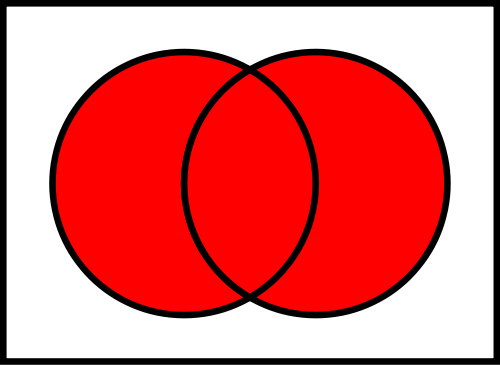
\includegraphics{AcupB}}
	\caption{Union}
	\end{subfigure}
&
	\begin{subfigure}{.25\textwidth}
	\resizebox{\linewidth}{!}{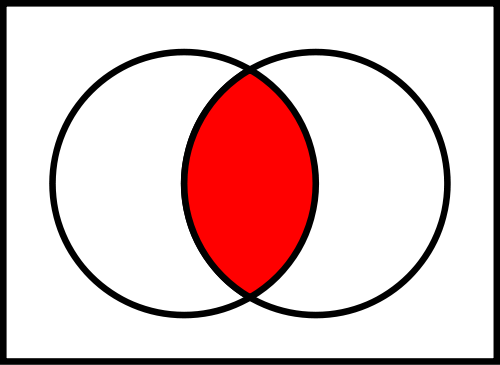
\includegraphics{AcapB}}
	\caption{Intersection}
	\end{subfigure}
&
	\begin{subfigure}{.25\textwidth}
	\resizebox{\linewidth}{!}{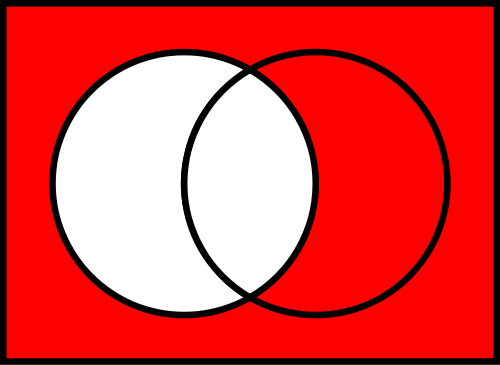
\includegraphics{Acomp}}
	\caption{Complement}
	\end{subfigure}
\end{tabular}
\end{figure}

\begin{table}
\centering
\caption{Correspondence with logical operators.}
\begin{tabular}{|c|c||c|c|c|} \hline
Set Theory 		& 			& Logic			&		& \\ \hline
Union			& $A\cup B$	& Disjunction 	& OR 	& $\lor$	\\
Intersection		& $A\cap B$	& Conjunction	& AND 	& $\land$\\
Complement		& $A^c$		& Negation		& NOT 	& $\lnot$	\\ \hline
\end{tabular}
\end{table}

%----------------------------------------------------------------------
\subsection{Set algebra}
%----------------------------------------------------------------------
\begin{definition}
\ben
\it Commutative property.
\bit 
\it $A\cup B = B\cup A$,
\it $A\cap B = B\cap A$.
\eit
\it Associative property.
\bit 
\it $(A\cup B)\cup C = A\cup (B\cup C)$,
\it $(A\cap B)\cap C = A\cap (B\cap C)$.
\eit
\it Distributive property.
\bit 
\it $A\cup (B\cap C) = (A\cup B)\cap(A\cup C)$,
\it $A\cap (B\cup C) = (A\cap B)\cup(A\cap C)$.
\eit
\een
\end{definition}

\begin{remark}
A statement such as $A\cup B\cap C$ is ambiguous. 
\end{remark}

%----------------------------------------------------------------------
\section{De Morgan's laws}
%----------------------------------------------------------------------
Union and intersection swap roles under complementation.

\begin{theorem}\label{thm:demorgan_simple}
\ben
\it $(A\cup B)^c = A^c\cap B^c$.
\it $(A\cap B)^c = A^c\cup B^c$.
\een
\end{theorem}

\begin{proof}
\begin{enumerate}
\item % part (1)
Let $a\in(A\cup B)^c$. Then $a\notin A$ and $a\notin B$, so $a\in A^c\cap B^c$.
Hence $(A\cup B)^c\subseteq A^c\cap B^c$.\par
Let $a\in A^c\cap B^c$. Then $a\notin A$ and $a\notin B$, so $a\notin A\cup B$.
Hence $A^c\cap B^c\subseteq (A\cup B)^c$.\par
Thus it follows that $(A\cup B)^c = A^c\cap B^c$.
\item % part (2)
Apply part (1) to the sets $A^c$ and $B^c$: $(A^c\cup B^c)^c = A\cap B$.\par
Then take the complement of both sides: $(A\cap B)^c = A^c\cup B^c$.
\end{enumerate}
\end{proof}

%----------------------------------------------------------------------
\section{Set difference}
%----------------------------------------------------------------------
\begin{definition}
Let $A$, $B$ and $\Omega$ be sets, with $A,B\subseteq \Omega$.
\ben
\it The \emph{set difference} between $A$ and $B$ is the set
$$
A\setminus B = \{a\in \Omega : a\in A \text{ and } a\notin B\}. % = A\cap B^c.
$$
\it The \emph{symmetric difference} between $A$ and $B$ is the set 
$$
A\bigtriangleup B = (A\setminus B) \cup (B\setminus A). %= (A\cap B^c)\cup (B\cap A^c). 
$$
\een
\end{definition}

\bit
\it $A\setminus B$ is the set of points that are in $A$ but not in $B$.
\it $A\bigtriangleup B$ is the set of points that are in either $A$ or $B$, but not both.
\eit

% example
\begin{example}
Let $A=\{a,b\}$ and $B=\{b,c\}$. Then
\bit
\it $A\setminus B = \{a\}$
\it $A\bigtriangleup B = \{a,c\}$.
\eit
\end{example}

%----------------------------------------------------------------------
%\section*{Appendix: Set operations}
%----------------------------------------------------------------------
% figure
\begin{figure}
\centering
\caption{Set Operations ($A$ on the left, $B$ on the right).\label{fig:set-operations}}
\begin{tabular}{cccc}	
\begin{subfigure}{.15\textwidth}
\resizebox{\linewidth}{!}{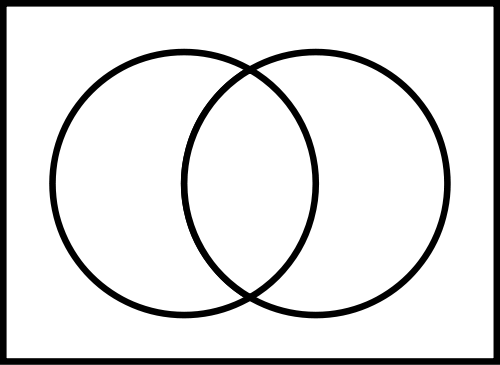
\includegraphics{emptyset}}
\caption{$\emptyset$}
\end{subfigure}
&
\begin{subfigure}{.15\textwidth}
\resizebox{\linewidth}{!}{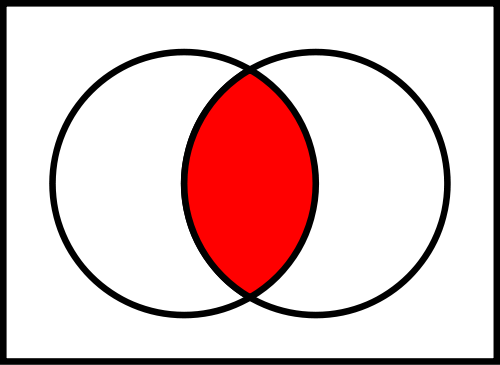
\includegraphics{AcapB}}
\caption{$A\cap B$}
\end{subfigure}
&
\begin{subfigure}{.15\textwidth}
\resizebox{\linewidth}{!}{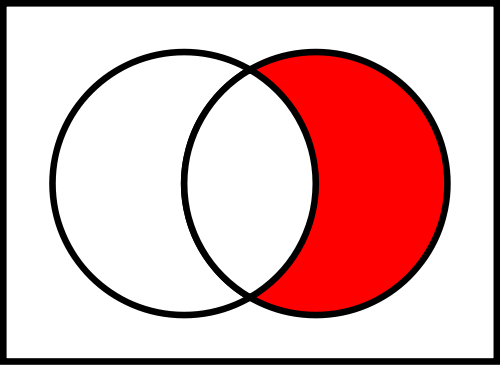
\includegraphics{BminusA}}
\caption{$B\setminus A$}
\end{subfigure}
&
\begin{subfigure}{.15\textwidth}
\resizebox{\linewidth}{!}{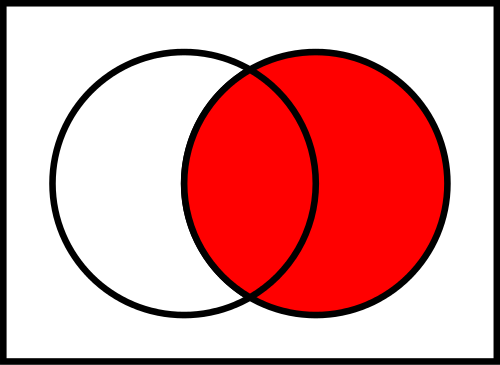
\includegraphics{setB}}
\caption{$B$}
\end{subfigure}
\end{tabular}

\begin{tabular}{cccc}
\begin{subfigure}{.15\textwidth}
\resizebox{\linewidth}{!}{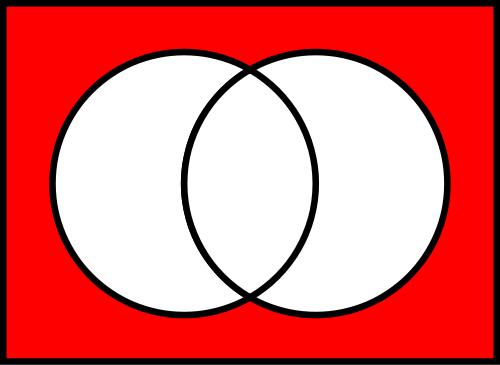
\includegraphics{AcupB_comp}}
\caption{$(A\cup B)^c$}
\end{subfigure}
&
\begin{subfigure}{.15\textwidth}
\resizebox{\linewidth}{!}{
\includegraphics{symdiff_comp}}
\caption{$(A\bigtriangleup B)^c$}
\end{subfigure}
&
\begin{subfigure}{.15\textwidth}
\resizebox{\linewidth}{!}{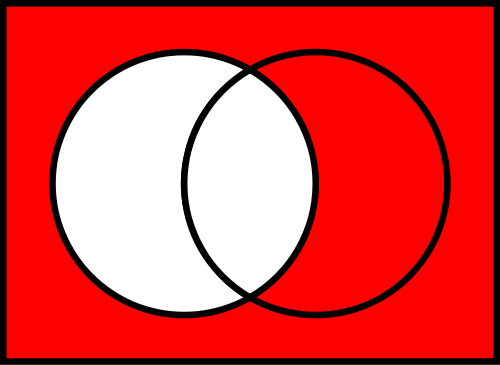
\includegraphics{Acomp}}
\caption{$A^c$}
\end{subfigure}
&
\begin{subfigure}{.15\textwidth}
\resizebox{\linewidth}{!}{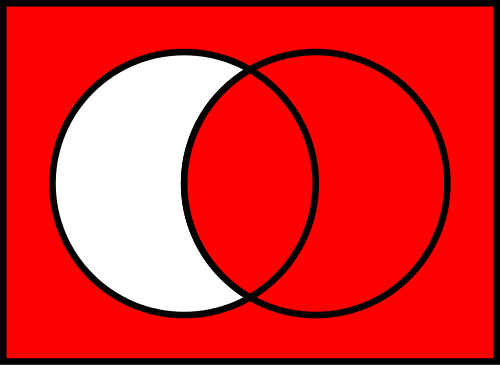
\includegraphics{AminusB_comp}}
\caption{$(A\setminus B)^c$}
\end{subfigure}
\end{tabular}

\begin{tabular}{cccc}
\begin{subfigure}{.15\textwidth}
\resizebox{\linewidth}{!}{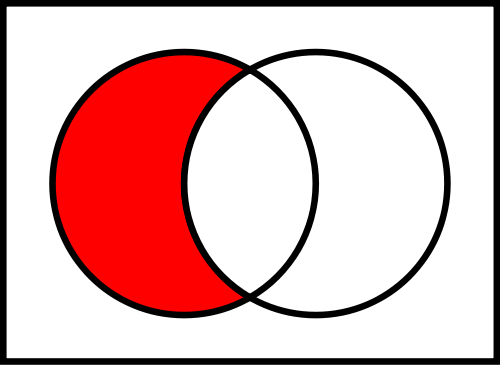
\includegraphics{AminusB}}
\caption{$A\setminus B$}
\end{subfigure}
&
\begin{subfigure}{.15\textwidth}
\resizebox{\linewidth}{!}{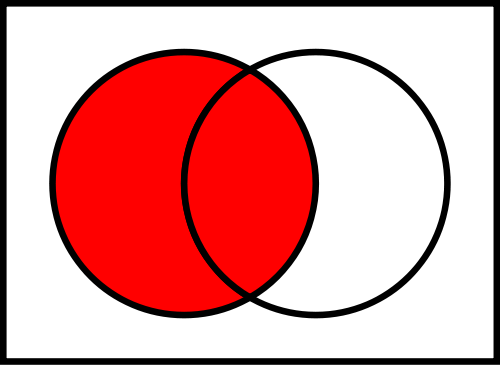
\includegraphics{setA}}
\caption{$A$}
\end{subfigure}
&
\begin{subfigure}{.15\textwidth}
\resizebox{\linewidth}{!}{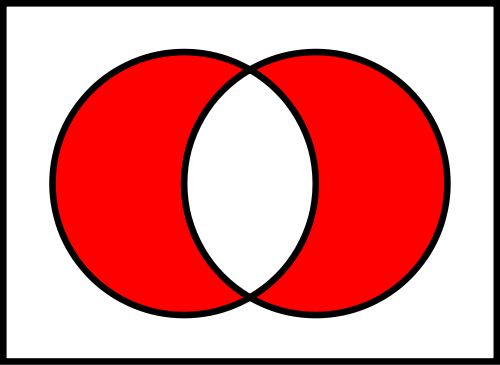
\includegraphics{symdiff}}
\caption{$A\bigtriangleup B$}
\end{subfigure}
&
\begin{subfigure}{.15\textwidth}
\resizebox{\linewidth}{!}{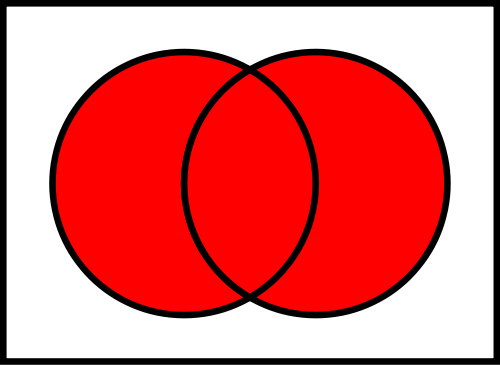
\includegraphics{AcupB}}
\caption{$A\cup B$}
\end{subfigure}
\end{tabular}

\begin{tabular}{cccc}
\begin{subfigure}{.15\textwidth}
\resizebox{\linewidth}{!}{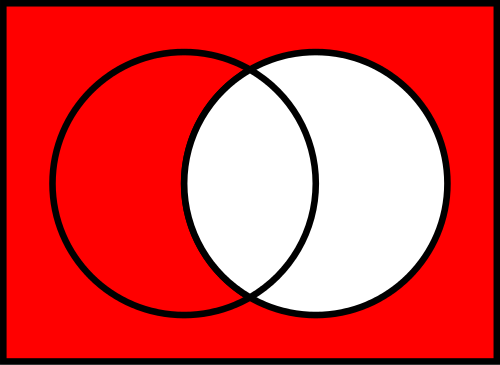
\includegraphics{Bcomp}}
\caption{$B^c$}
\end{subfigure}
&
\begin{subfigure}{.15\textwidth}
\resizebox{\linewidth}{!}{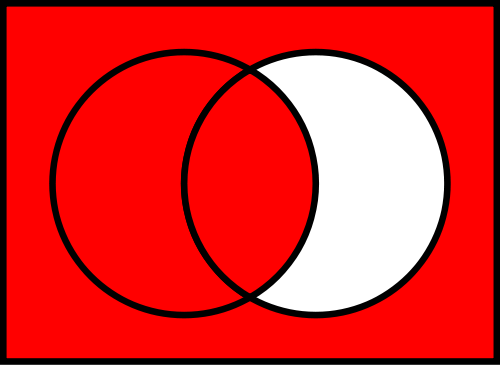
\includegraphics{BminusA_comp}}
\caption{$(B\setminus A)^c$}
\end{subfigure}
&
\begin{subfigure}{.15\textwidth}
\resizebox{\linewidth}{!}{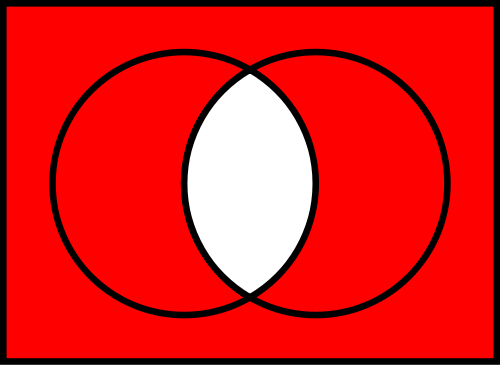
\includegraphics{AcapB_comp}}
\caption{$(A\cap B)^c$}
\end{subfigure}
&
\begin{subfigure}{.15\textwidth}
\resizebox{\linewidth}{!}{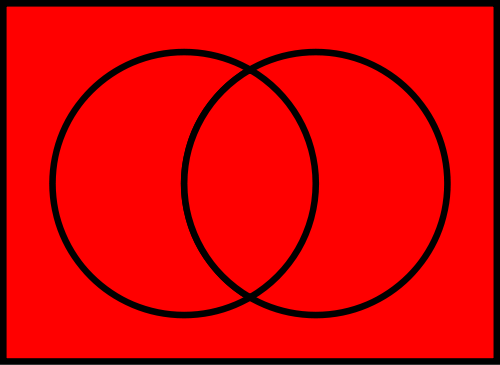
\includegraphics{universe}}
\caption{$\emptyset^c$}
\end{subfigure}
\end{tabular}
\end{figure}

%----------------------------------------------------------------------
\section{Assessment}
%----------------------------------------------------------------------

\begin{assessment}
\begin{questions}
\question
Illustrate the basic set operations using Venn diagrams.%, as shown in Figure~\ref{fig:set-operations}.
\question
State and prove De Morgan's laws.
\end{questions}
\end{assessment}

%======================================================================
\endinput
%======================================================================
